\documentclass[11pt,a4paper,oneside]{report}
\usepackage{geometry}
\usepackage{fancyhdr}
\usepackage[ngerman]{babel}
\usepackage{bpchem}
\usepackage{fontspec}
\usepackage[compact]{titlesec}
\usepackage[numbers]{natbib}
\usepackage{url}
\usepackage{amsmath}
\usepackage{amsfonts}
\usepackage[german, plain]{fancyref}
\usepackage{tocloft}


\setmainfont{Arial}
\titleformat{\chapter}[hang]{\LARGE\bfseries}{\thechapter}{1em}{}
\titleclass{\chapter}{straight}
\bibliographystyle{apa}
\renewcommand{\baselinestretch}{1.5}
\geometry{
a4paper,
total={170mm,257mm},
left=25mm,
top=20mm
}

\begin{document}
\pagestyle{empty}
\includegraphics[scale=0.75]{FacharbeitTittelblattT.pdf}

\newpage

\titlespacing{\chapter}{0em}{1em}{1.5em}[0pt]
\renewcommand{\contentsname}{Inhaltsverzeichnis}
%\renewcommand{\bibname}{\section{Quellen}}
\renewcommand{\bibname}{Quellen}
\setlength{\parindent}{0em}

\pagestyle{fancy}
\fancyhf{}
\fancyhead[CEO]{\thepage}
\renewcommand{\headrulewidth}{0pt}

\renewcommand{\cftdot}{}

\setcounter{page}{2}

% Content

\tableofcontents

\clearpage

\chapter{Einleitung und Vorbetrachtung}

Glas, also \BPChem{SiO\_2}, ist einer der wenigen Feststoffe, die für sichtbares Licht durchlässig sind. Diese Facharbeit möchte rechnerisch aufzeigen, warum Glas das sichtbare Licht durchlässt. Dazu sollen die Theorien der Quantenmechanik herangezogen werden. Stoffe sind undurchlässig für Licht und andere elektromagnetische Wellen, wenn sie elektrisch oder magnetisch mit diesen interagieren. Zur Betrachtung dieses Umstandes müssen drei Modelle herangezogen werden\cite{pape99}.

\chapter{Beschreibung der physikalisch-chemischen Modelle}
Im Folgenden sollen die Modelle beschrieben werden, die zur Erklärung des in der Einleitung beschriebenen Effekts notwendig sind.

\section{Modelle der Quantenmechanik}
In der Quantenmechanik wird angenommen, dass alle Elementarteilchen sowohl Teilchen- als auch Wellencharakter haben. Außerdem haben auch die bis dahin nur als Feld beschriebenen Effekte Teilchencharakter, zum Beispiel das elektromagnetische Feld, das durch Photonen übertragen wird. Für diese Arbeit ist allerdings nur ein Teil der Quanten relevant, dies sind:
\begin{table}[ht]
\centering
\begin{tabular}{|l|lr|} \hline
Teilchen 				& Eigenschaften 	&  						\\  \hline
Elektron( $e^-$ ) 		& Masse: 			& $m_e=9,109*10^{-31}kg$	\\
					& Ladung: 		& $-e=-1,602*10^{-19}C$	\\ \hline
Proton($p^+$) 		& Masse: 			& $m_p=1,672*10^{-27}kg$ 	\\
 					& Ladung: 		& $e=1,602*10^{-19}kg$	\\ \hline 
Neutron($N$)			& Masse:			& $m_N=1,674*10^{-27}C$	\\ 
					& Ladung:		& $0$					\\ \hline
Photon($ \lambda $) 	& Masse: 			& $0$					\\ 
					&Ladung:			& $0$					\\ \hline
\end{tabular}
\caption{Die zur Betrachtung notwendigen Teilchen\cite[S. 433]{stroppe08}}.
\end{table}

\subsection{Das Elektron}
Das Elektron ist das kleinste und leichteste der Elementarteilchen. Es ist negativ mit einer Elementarladung($e$) geladen und besitzt die Masse($m_e$). In den meisten Fällen wird ein elektrischer Strom durch Elektronen übertragen. Elektronen bilden zusammen mit den Protonen und den Neutronen Atome, wobei die Elektronen die Atomschale bilden.

\subsection{Das Proton}
Das Proton selbst ist kein Quantum, sondern besteht aus drei kleineren Quanten, diese sind allerdings nicht alleine beobachtbar. Das Proton hat eine positive Elementarladung($e$) und eine wesentlich größere Masse($m_p$) als das Elektron. Es bildet zusammen mit den Neutronen den Atomkern.

\subsection{Das Neutron}
Das Neutron ist wie das Proton kein Quantum, sondern besteht auch aus drei kleineren Quanten. Es hat eine noch größere Masse($m_N$) als das Proton, ist allerdings nicht geladen.

\subsection{Das Photon}
Das Photon ist ein Wirkungsquantum und besitzt als solches weder Masse noch eine Ladung. Das Photon übermittelt als Wirkungsquantum das elektromagnetische Feld.Die Energie des Photons ergibt sich aus: 

\begin{figure}[ht]
\centering
$E=hf \text{\hspace{1em} mit \hspace{1em}} h=6,626069*10^{-34}Js$
\caption{Die Energie eines Photons\cite[S. 421]{stroppe08}}
\end{figure}

\section{Orbitalmodell und erweitertes Orbitalmodell}
Das Bohrsche Atommodell beschreibt ein Atom ähnlich unserem Sonnensystem. Dabei steht der Atomkern im Zentrum und wird von den Elektronen umkreist. Im Kern befinden sich die Protonen und die Neutronen. Zur Kategorisierung von Atomen wird die Anzahl der Protonen im Kern verwendet. Diese entspricht bei einem neutralen Atom auch der Anzahl der Elektronen. Die Elektronen umkreisen den Atomkern dabei auf bestimmten Bahnen auch Hauptenergieniveaus(n) genannt\cite{hefterCh}.

\subsection{Orbitalmodell}
Im Orbitalmodell gibt es innerhalb der Hauptenergieniveaus Unterniveaus(l), die sich auch energetisch voneinander unterscheiden. Die Unterniveaus wiederum bestehen aus energetisch gleichen, aber räumlich unterschiedlichen Orbitalen. Diese wiederum können je zwei Elektronen mit den Spinquantenzahlen($s$) $+\frac{1}{2}$ und $-\frac{1}{2}$\cite{hefterCh} enthalten.
\\
Es sind fünf Unterenergieniveaus bekannt, dies sind in der Reihnfolge ihrer l-Werte s, p, d, f und g wobei s den l-Wert 0 hat und dieser immer um eins zunimmt.

\begin{table}[ht]
\centering
\begin{tabular}{|c|c|c|c|} \hline
Hauptenergieniveau 	& Unterenergieniveau 	& Anzahl der Orbitale	&Position im Energieniveauschema	\\ \hline
1					&s					&1					&1								\\ \hline
2					&s					&1					&2								\\ 
					&p					&3					&3								\\ \hline
3					&s					&1					&4								\\
					&p					&3					&5								\\
					&d					&5					&7								\\ \hline
4					&s 					&1					&6								\\
					&p 					&3					&8								\\
					&d 					&5					&10								\\
					&f 					&7					&13								\\ \hline
\end{tabular}
\caption{Aufgliederung der ersten vier Hauptenergieniveaus \cite[Umschlag]{tw}}
\end{table}

\subsection{Erweitertes Orbitalmodell}

Unter bestimmten Umständen kommt es dazu, dass ein Atom, das eigentlich eine geringe Bindigkeit hat, eine höhere Bindigkeit besitzt, da diese energetisch günstiger ist. Zum Beispiel Methan(\BPChem{CH\_4}), wo der eigentlich zweibindige Kohlenstoff vierbindig ist. Dies lässt sich am besten dadurch erklären, dass der Kohlenstoff seine 2s und 2p Orbitale hybridisiert.
\\
Bei der Hybridisierung werden Orbitale, die energetisch und räumlich ungleichartig, sind zu energetisch und räumlich gleichartigen Hybridorbitalen. Dazu wird zuerst ein Elektron aus einem vollen Orbital in ein leeres energetisch höheres  Orbital verschoben. Dann werden diese energetisch und räumlich angeglichen. Dabei entstehen Hybridorbitale, die insgesamt energetisch und räumlich den Ausgangsorbitalen entsprechen\cite[S. 100ff]{riedel08}. Das Energieniveau eines Orbitals ergibt sich aus:
\\
\begin{figure}[ht]
\centering
$E_n=-\frac{e^4m_e}{8\epsilon_0^2h^2}\frac{Z^2}{n^2}=-13,6\frac{Z^2}{n^2}eV$
\caption{Die Berechnung eines Energieniveaus\cite[S.439]{stroppe08}}
\label{fig:energieniveauberechnung}
\end{figure}
\\
$Z$ bezeichnet die Kernladungszahl und $n$ die Hauptquantenzahl. Dabei gibt es innerhalb dieses Hauptenerginiveaus noch energetisch und räumlich geringfügig unterschiedliche Unterenergieniveaus. Die Energiedifferenz zwischen dem Hauptenergieniveau und dem Unterenergieniveau ist so gering, dass sie im Rahmen dieser Arbeit vernachlässigt werden kann.

\section{Photon-Elektron-Reaktion(Photoeffekt)}

Der Photoeffekt, oder auch lichtelektrischer Effekt, beschreibt die Aufnahme eines Photons durch ein Elektron, wobei dieses die Energie des Photons aufnimmt.\cite{stroppe08} Dabei wird das Elektron beschleunigt, da der Energieerhaltungssatz($E_{in}=E_{out}$) erfüllt werden muss. 

Photonen reagieren allerdings nur mit einem gebundenen Elektron, wenn sie dieses entweder in ein höheres Energieniveau oder ganz aus dem Atom heben können. Dies schränkt die Interaktionen von Photonen mit Materie in dieser Weise extrem ein. Um ein Elektron aus einem Atom zu lösen, muss die Differenz zwischen $E_\infty$ und $E_n$ aufgebracht werden.
\begin{figure}[ht]
\centering
$E_{\infty} = \lim\limits_{n \to \infty} -13,6\frac{Z^2}{n^2} eV= 0eV$
 \caption{Berechnung des Energieniveaus für ungebundene Elektronen\cite[S. 439]{stroppe08}}
\end{figure}

\section{Compton-Effekt}
Der Compton-Effekt ist ähnlich des Photoeffekts eine Reaktion von Photonen mit Elektronen, wobei hier nur ein Teil der Energie des Photons vom Elektron aufgenommen wird. Daraus ergibt sich aber auch die größte Einschränkung dieses Modells, es trifft meist nur auf sehr kurzwellige Strahlung wie ultraviolette Strahlung zu\cite{stroppe08}, da das Photon das Elektron zumindest um ein Energieniveau anheben muss, wenn danach noch Energie in Form eines Photons emittiert werden soll.

\section{Paarbildung}
Bei der Paarbildung entstehen aus einem Photon zwei gegensätzlich geladene Teilchen, aufgrund des Impulserhaltungssatzes wird dazu ein geladenes Teilchen benötigt, welches den nicht durch das Photon gedeckten Gegenimpuls aufnimmt. In den meisten Fällen ist dies ein Atomkern, in dessen Coulomb-Feld die Paarbildung stattfindet. Da allerdings auch der Energieerhaltungssatz erfüllt werden muss, hat das betreffende Photon mindestens eine Energie so groß wie die Ruhemasse der erzeugten Teilchen.
\begin{figure}[ht]
\centering
$E_{\lambda} = 2m_Rc^2$
 \caption{Energie Photons für die Paarbildung\cite[S. 457f]{stroppe08}}
\end{figure}

Das kleinste Teilchen, das bei diesem Vorgang entstehen kann, ist das Elektron, was die minimale Energie des Photons($E_{\lambda_{min}}$) auf $1,022MeV$ hebt\cite[S.458]{stroppe08}. Diese Energie ist um drei Größenordnungen größer, als die des sichtbaren Lichts, was diesen Effekt für das Thema dieser Arbeit irrelevant macht.

\section{Sichbares Licht}
Der Ausdruck sichtbares Licht beschreibt elektromagnetische Wellen mit Wellenlängen zwischen $390nm$ und $780nm$. Es ist das für das menschliche Auge sichtbare Spektrum der elektromagnetischen Wellen.

\pagebreak

\chapter{Rechnerischer Nachweis}

Durch die Anwendung der in \Fref{fig:energieniveauberechnung} beschriebenen Berechnungsvorschrift erhält man für den Sauerstoff und das Silicium folgende Energiniveaus:
\begin{table}[ht]
\centering
\begin{tabular}{|l|r|r|}
\hline
Hauptquantenzahl&Energie von \BPChem{O} in $eV$& Energie von \BPChem{Si} in $eV$ \\ \hline
1&-870,4000 &-2665,6000\\ \hline
2&-217,6000&-666,4000 \\ \hline
3&-96,7111&-296,1778 \\ \hline
4&-54,4000&-166,6000 \\ \hline
5&-34,8160 &-106,6240 \\ \hline
6&-24,1778&-74,0444 \\ \hline
7&-17,7633&-54,4000 \\ \hline
8&-13,6000 & -41,6500\\ \hline
9&-10,7457 & -32,9086 \\ \hline
10&-8,7040&-26,6560 \\ \hline
100&-0,0870 & -0,2666 \\ \hline
1000&-0,0009 & -0,0027 \\ \hline
10000&0,0000& 0,0000 \\ \hline
\end{tabular}
\caption{Eine Auswahl der Energieniveaus des Sauerstoff- und Siliciumatoms}
\label{tab:ENiveaus}
\end{table}

Wenn man nun die Differenzen aus den in \Fref{tab:ENiveaus} ermittelten Energien bildet, erhält man die wahrscheinlichsten Spektrallinien der beiden Elemente. Diese kann man nun mit dem Spektrum des sichtbaren Lichts vergleichen. Daraus erhält man die in \Fref{fig:ENSi} und \Fref{fig:ENO} dargestellten Ergebnisse. Die beiden Datenpunkte, die beim Sauerstoff im Spektrum des sichtbaren Lichts liegen, sind die Übergänge vom zehnten zum neunten, beziehungsweise vom neunten zum achten Hauptenergieniveau. Da diese weit außerhalb der im nicht angeregten Zustand belegten Hauptenergieniveaus liegen, sind hier meist keine Elektronen, die mit Photonen interagieren könnten.

\pagebreak

\begin{figure}[ht]
\centering
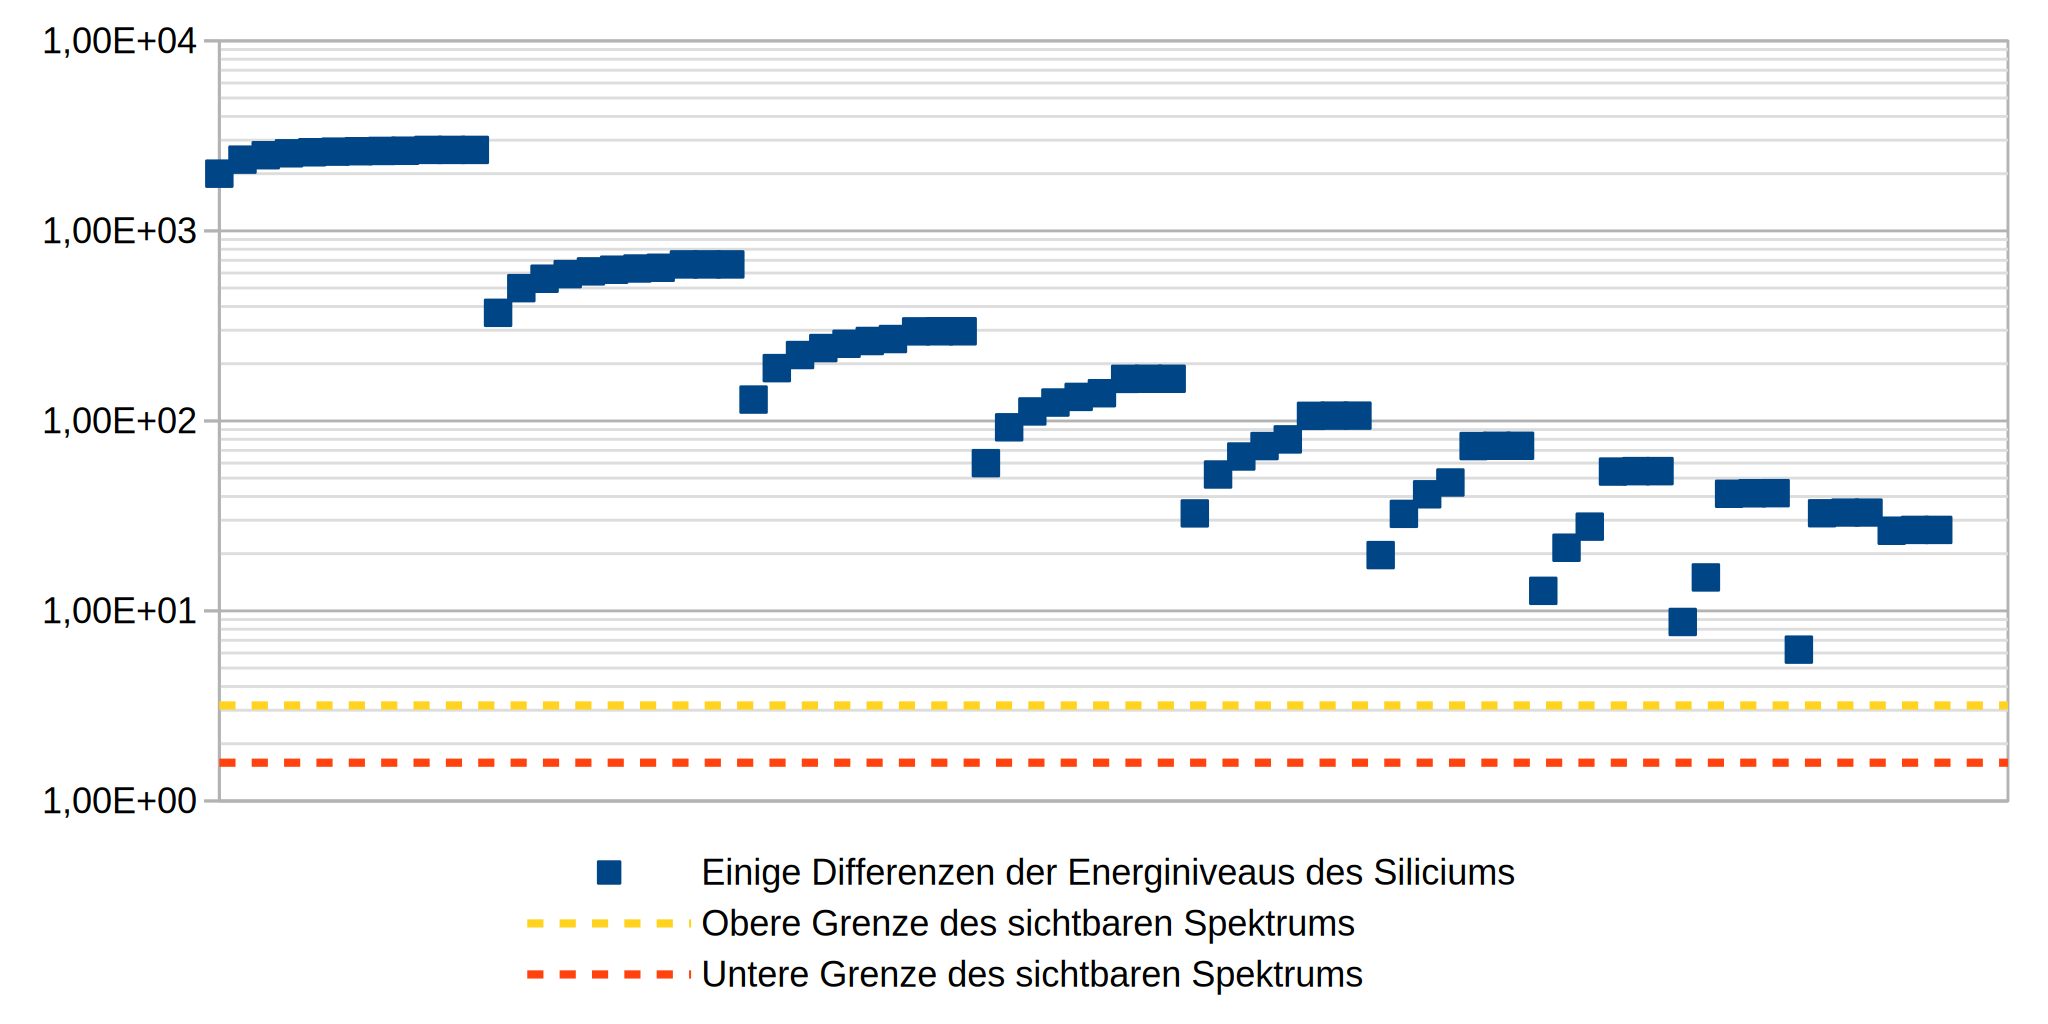
\includegraphics[scale=0.7]{SiliciumENiveaus.pdf}
\caption{Die Differenzen der Energieniveaus im Siliciumatom im Vergleich zum Energiegehalt von sichtbarem Licht}
\label{fig:ENSi}
\end{figure}

\begin{figure}[ht]
\centering
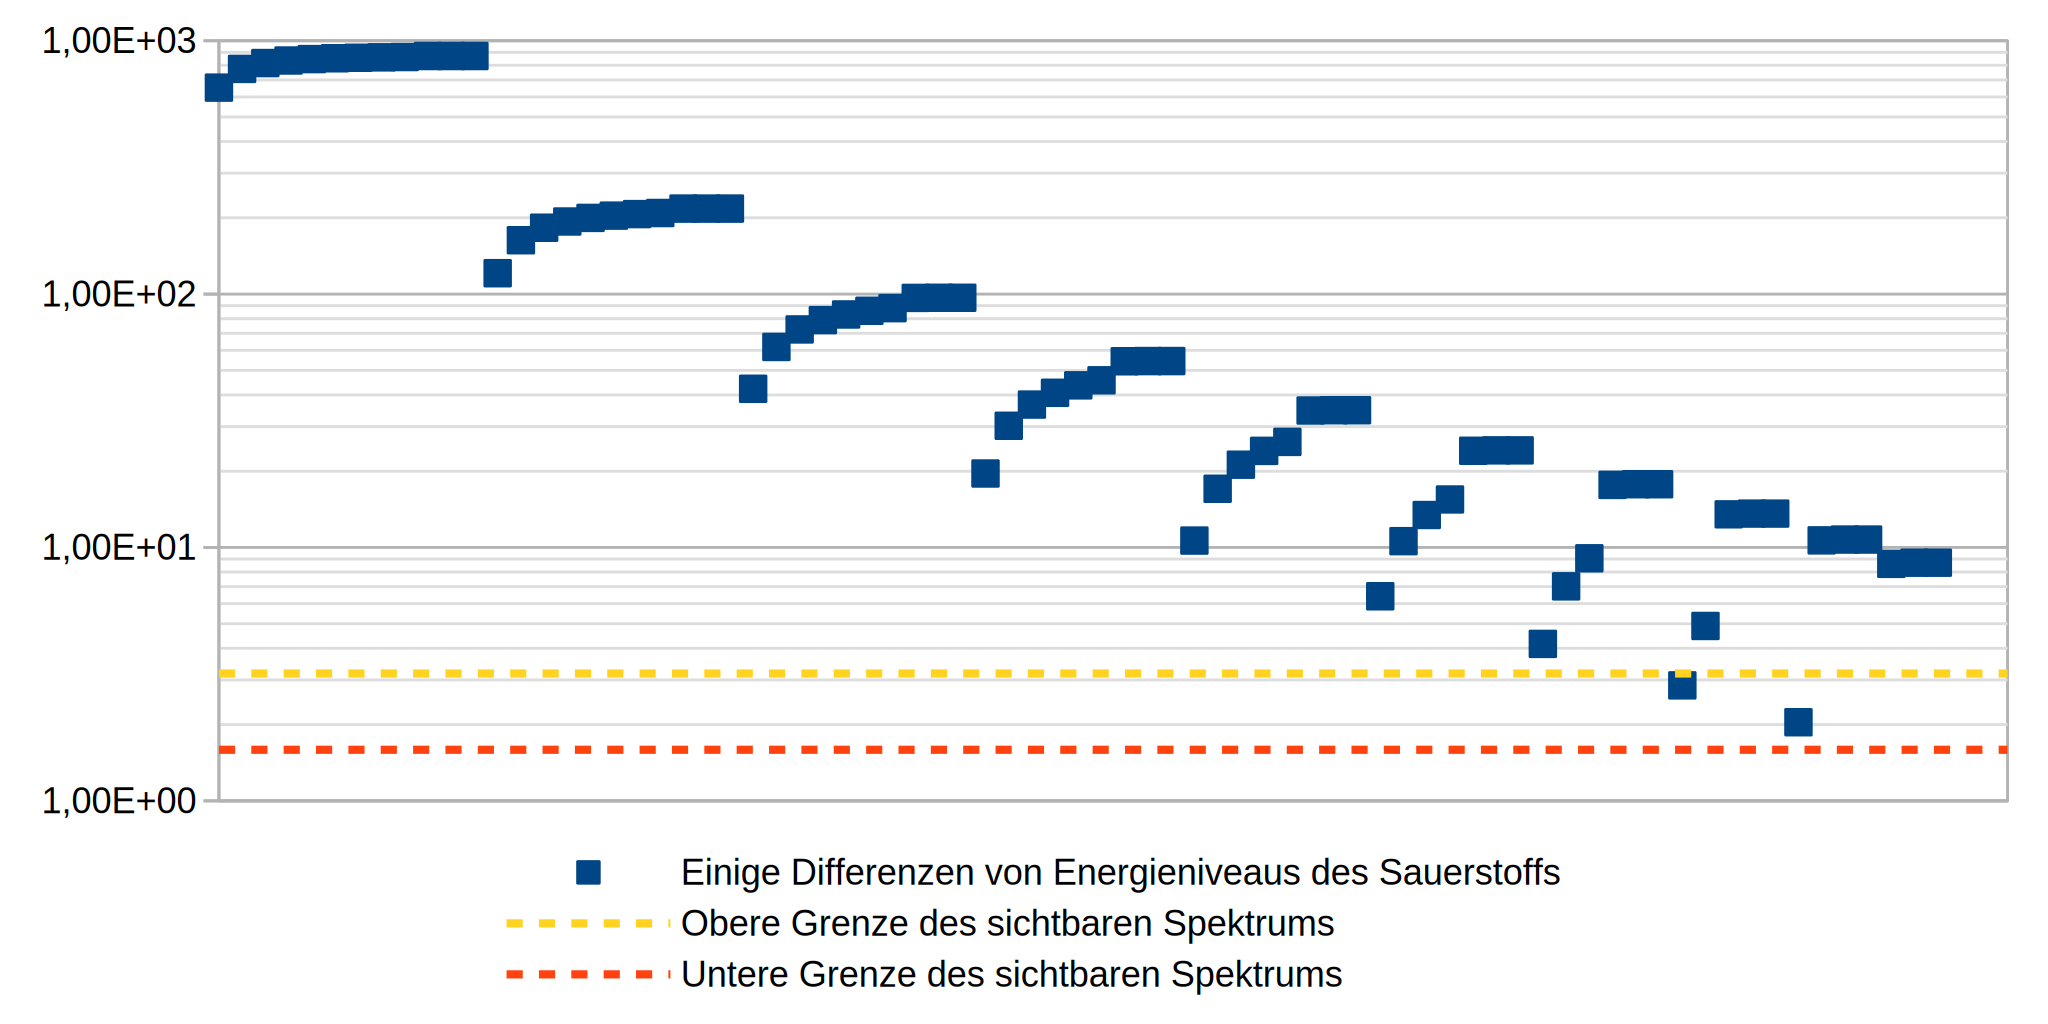
\includegraphics[scale=0.7]{SauerstoffENiveaus.pdf}
\caption{Die Differenzen der Energieniveaus im Sauerstoffatom im Vergleich zum Energiegehalt von sichtbarem Licht}
\label{fig:ENO}
\end{figure}

\iffalse

\begin{table}[ht]
\centering
\begin{tabular}{|c|c|c|c|c|c|c|c|c|c|c|c|c|}
-2665.6&-666.4&-296.18&-166.6&-106.62&-74.04&-54.4&-41.65&-32.91&-26.66&-0.27&-0.0027&-0.000027 \\ \hline \hline
-&1999.2&2369.42&2499&2558.98&2591.56&2611.2&2623.95&2632.69&2638.94&2665.33&2665.6&2665.6\\ \hline
&-&370.22&499.8&559.78&592.36&612&624.75&633.49&639.74&666.13&666.4&666.4\\ \hline
&&-&129.58&189.56&222.13&241.78&254.53&263.27&269.52&295.91&296.18&296.18\\ \hline
&&&-&59.98&92.56&112.2&124.95&133.7&139.94&166.33&166.6&166.6\\ \hline
&&&&-&32.58&52.224&64.97&73.72&79.98&106.36&106.62&106.62\\ \hline
&&&&&-&19.64&32.39&41.14&47.39&73.78&74.04&74.04\\ \hline
&&&&&&-&12.75&21.49&27.74&54.13&54.4&54.4\\ \hline
&&&&&&&-&8.74&15&41.38&41.65&41.65\\ \hline
&&&&&&&&-&6.25&32.64&32.91&32.91\\ \hline
&&&&&&&&&-&26.39&26.65&26.66\\ \hline
&&&&&&&&&&-&0.26&0.27\\ \hline
&&&&&&&&&&&-&0.0026\\ \hline
\end{tabular}
\end{table}

\fi


\chapter{Schlussbetrachtung}
Aus diesen Berechnungen lässt sich schließen, dass das sichtbare Licht nicht mit Glas interagiert, da die einzigen Energiedifferenzen, die im Spektrum des sichtbaren Lichts liegen, zwischen dem achten und neunten, beziehungsweise dem neunten und zehnten Energieniveau des Sauerstoffs bestehen. Da diese aber im Normalfall nicht besetzt sind, kommt es so gut wie nie dazu, dass ein Photon mit Glas interagiert. Dies erklärt dann, warum Glas durchsichtig ist; weil das sichtbare Licht nicht mit Glas interagiert.

\clearpage

\pagestyle{empty}

\appendix{\chapter*{Anhang}}

\listoftables

\listoffigures

\bibliography{Sources}

\newpage

\pagestyle{empty}

\includegraphics[scale=0.75]{Selbständigkeitserklärung.pdf}


\end{document}